\documentclass{beamer}

\usetheme[aspectratio=169]{Dresden}
\definecolor{cerulean}{rgb}{0.0, 0.48, 0.65}
%\definecolor{darkcyan}{rgb}{0.0, 0.55, 0.55}
\usecolortheme[named=cerulean]{structure}

\fontfamily{cmr}\selectfont

\usepackage{ragged2e}
\usepackage[brazilian]{babel}
\usepackage{graphicx}
\usepackage[authoryear]{natbib}
\usepackage{hyperref} 
%\usepackage{subfig}
%\usepackage{amssymb,amsfonts,amsmath,amsthm,euscript}
\usepackage{indentfirst}
%\usepackage{ulem}
\usepackage{dsfont}
%\usepackage{placeins}
%\usepackage{enumitem}

\newcommand{\R}{\mathds{R}}
\newcommand{\N}{\mathds{N}}
\newcommand{\B}{\mathds{B}}
\newcommand{\Perp}{\mathcal{P}}
\newcommand{\bs}[1]{\boldsymbol{#1}}

\newcommand{\red}[1]{\textcolor{red}{#1}}
\newcommand{\blue}[1]{\textcolor{blue}{#1}}


\title{Composição Automática de Músicas utilizando Redes Neurais Recorrentes}
\author[Hahn, N. M.]{Nicolas Mathias Hahn \\ \footnotesize Orientador: Guilherme Pumi}
\institute[IME-UFRGS]{Departamento de Estatística \\ Instituto de Matemática e Estatística \\ Universidade Federal do Rio Grande do Sul (UFRGS)}
\date{Outubro de 2022 \\ \tiny Porto Alegre - RS}

\begin{document}

    \begin{frame}
        \maketitle
    \end{frame}


\section{Introdução}
    \begin{frame}{Contextualização}
        \begin{columns}[onlytextwidth,t]
            \begin{column}{0.48\textwidth}
                \centering
                \begin{itemize}
                    \justifying
                    \item Composição algorítmica refere-se ao processo de criação de músicas com o mínimo de intervenção humana.
                    \item A obra \textit{Musikalisches Wurfelspiel} (\textit{Dice Music}), de Wolfgang Amadeus Mozart (1756-1791), utilizou tal processo.
                \end{itemize}
            \end{column}
            \begin{column}{0.48\textwidth}
                \centering
                \vspace{-1cm}
                \begin{figure}
                    \includegraphics[scale=0.32]{figuras/dice_music.PNG}
                    \caption{\textit{Dice Music}}
	            \end{figure}
            \end{column}
        \end{columns}
    \end{frame}
    
    \begin{frame}{Contextualização}
        \begin{columns}[onlytextwidth,t]
            \begin{column}{0.5\textwidth}
                \centering
                \vspace{-0.5cm}
                \begin{figure}
                    \includegraphics[scale=0.32]{figuras/reunion_board.PNG}
                    \caption{Tabuleiro de Xadrez com Foto Receptor}
	            \end{figure}
            \end{column}
            \begin{column}{0.46\textwidth}
                \centering
                \begin{itemize}
                    \justifying
                    \item A performance \textit{Reunion}, de John Cage (1912-1992), também utilizou composição automática.
                    \item David Cope (1941-), em 1981, criou o EMI (\textit{Experiments in Musical Intelligence}), um sistema com descrições de estilos composicionais capaz de criar os próprios.
                \end{itemize}
            \end{column}
        \end{columns}
    \end{frame}

    \begin{frame}{Literatura}
        \begin{itemize}
            \justifying
            \item Via de regra, o problema de composição musical automática é explorado com foco na composição musical em si.
            \item Detalhes técnicos como os impactos que as modificações nos parâmetros têm na composição final, ainda, são amplamente desconhecidos.
            \item Exemplos: \citet{agarwala2017}, \citet{kuang2021}.
        \end{itemize}
    \end{frame}
    
    \begin{frame}{Objetivos}
        \begin{itemize}
            \justifying
            \item Estudar o quão sensível é um modelo de rede neural, baseado em processamento de linguagem natural, construído para composição musical.
            \item A mensuração será feita com a perplexidade, uma medida oriunda da teoria da informação.
            \item Avaliar, de forma subjetiva, as peças musicais obtidas em relação à musicalidade e à qualidade.
        \end{itemize}
    \end{frame}



\section{Referencial Teórico}
    \begin{frame}{RNA - Redes Neurais Artificiais}
        \begin{itemize}
            \justifying
            \item RNAs são técnicas de \textit{machine learning} inspiradas no mecanismo de aprendizagem de organismos vivos \citep{aggarwal2018}. 
            \item Nos seus primórdios, os algoritmos tinham o intuito de ser um modelo computacional capaz de imitar a aprendizagem ocorrida no cérebro \citep{goodfellow2016}.
            \item São constituídas por três tipos de camadas: entrada, oculta e saída.
        \end{itemize}
    \end{frame}

    \begin{frame}{RNA - Neurônio}
        \begin{figure}
            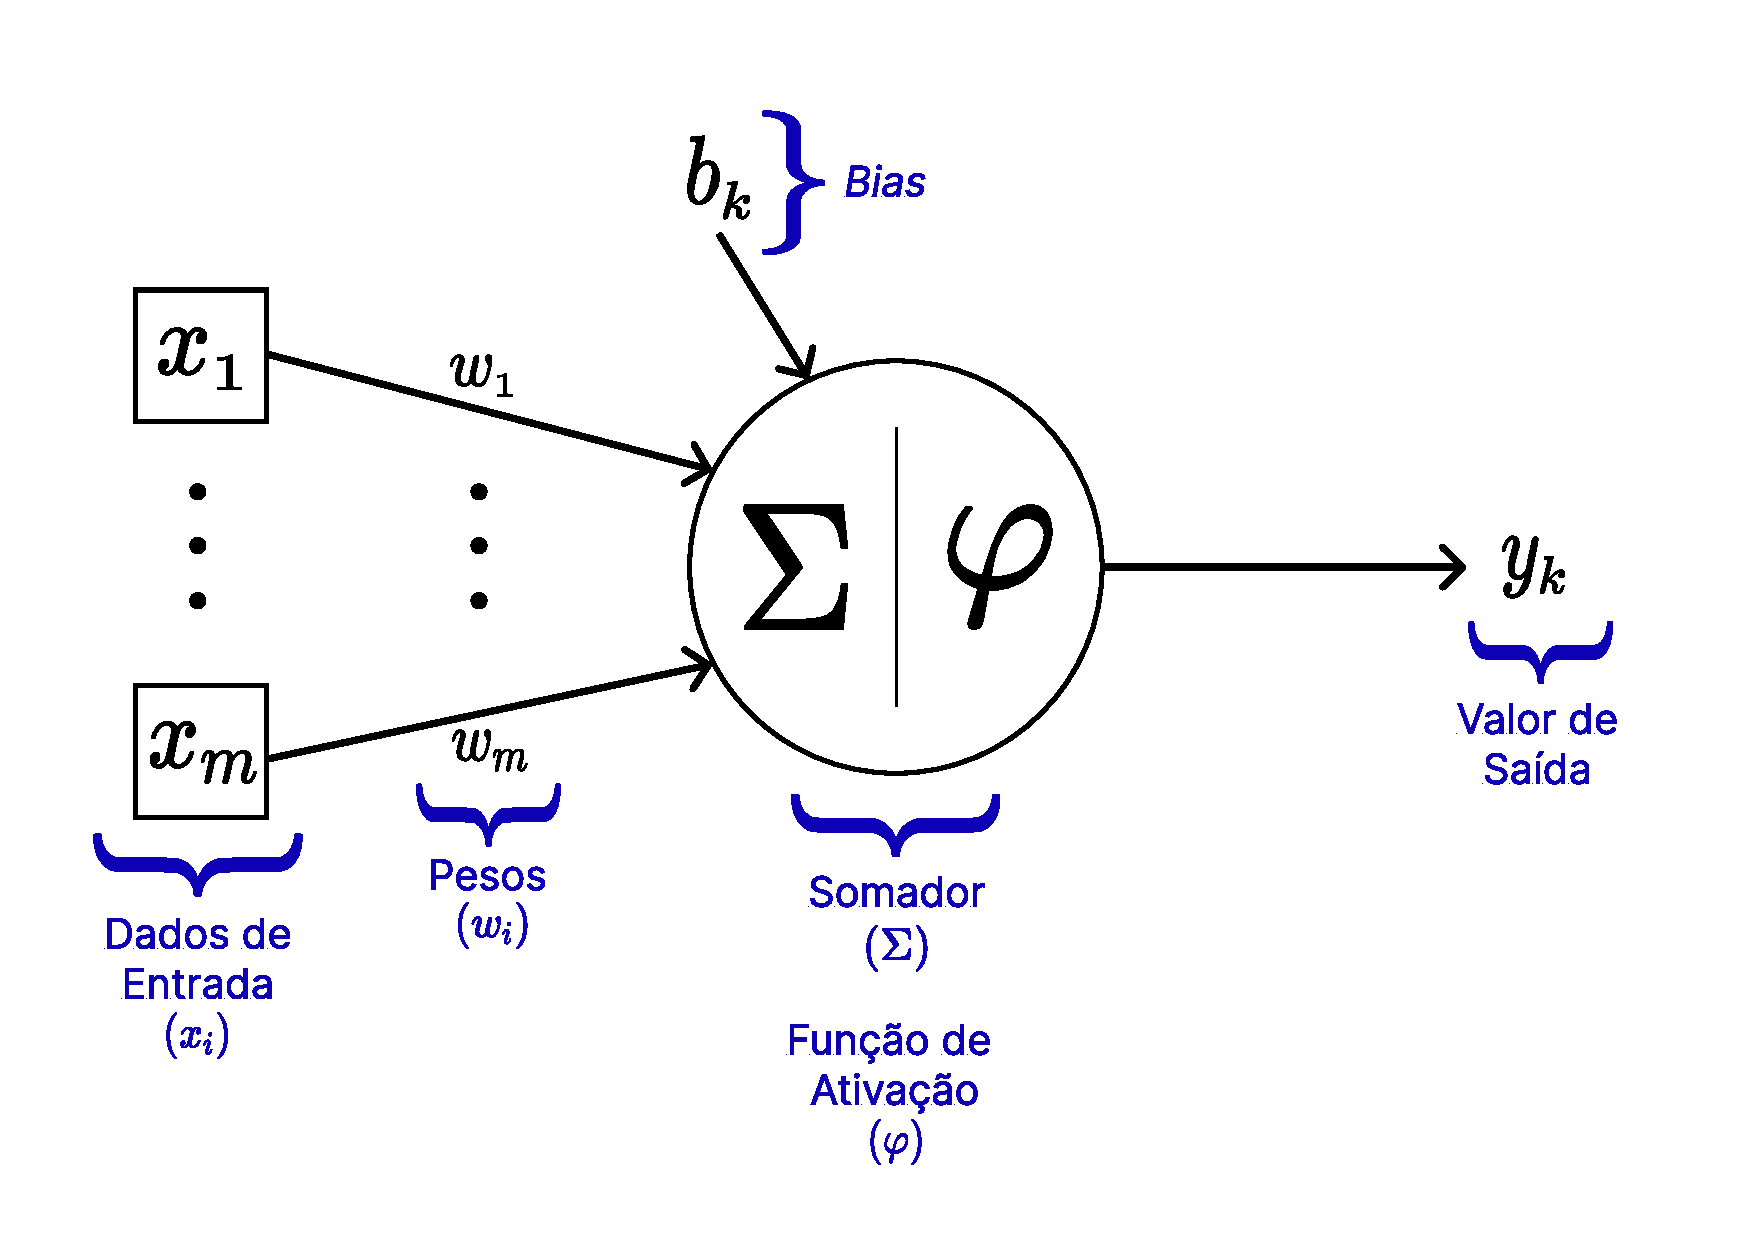
\includegraphics[scale=0.25]{figuras/neuron_model.pdf}
		    \caption{Modelo Neuronal \citep[adaptado de][]{hair2005,haykin2009}}
	    \end{figure}
    \end{frame}

    \begin{frame}{RNA - Rede Neural}
        \begin{figure}
            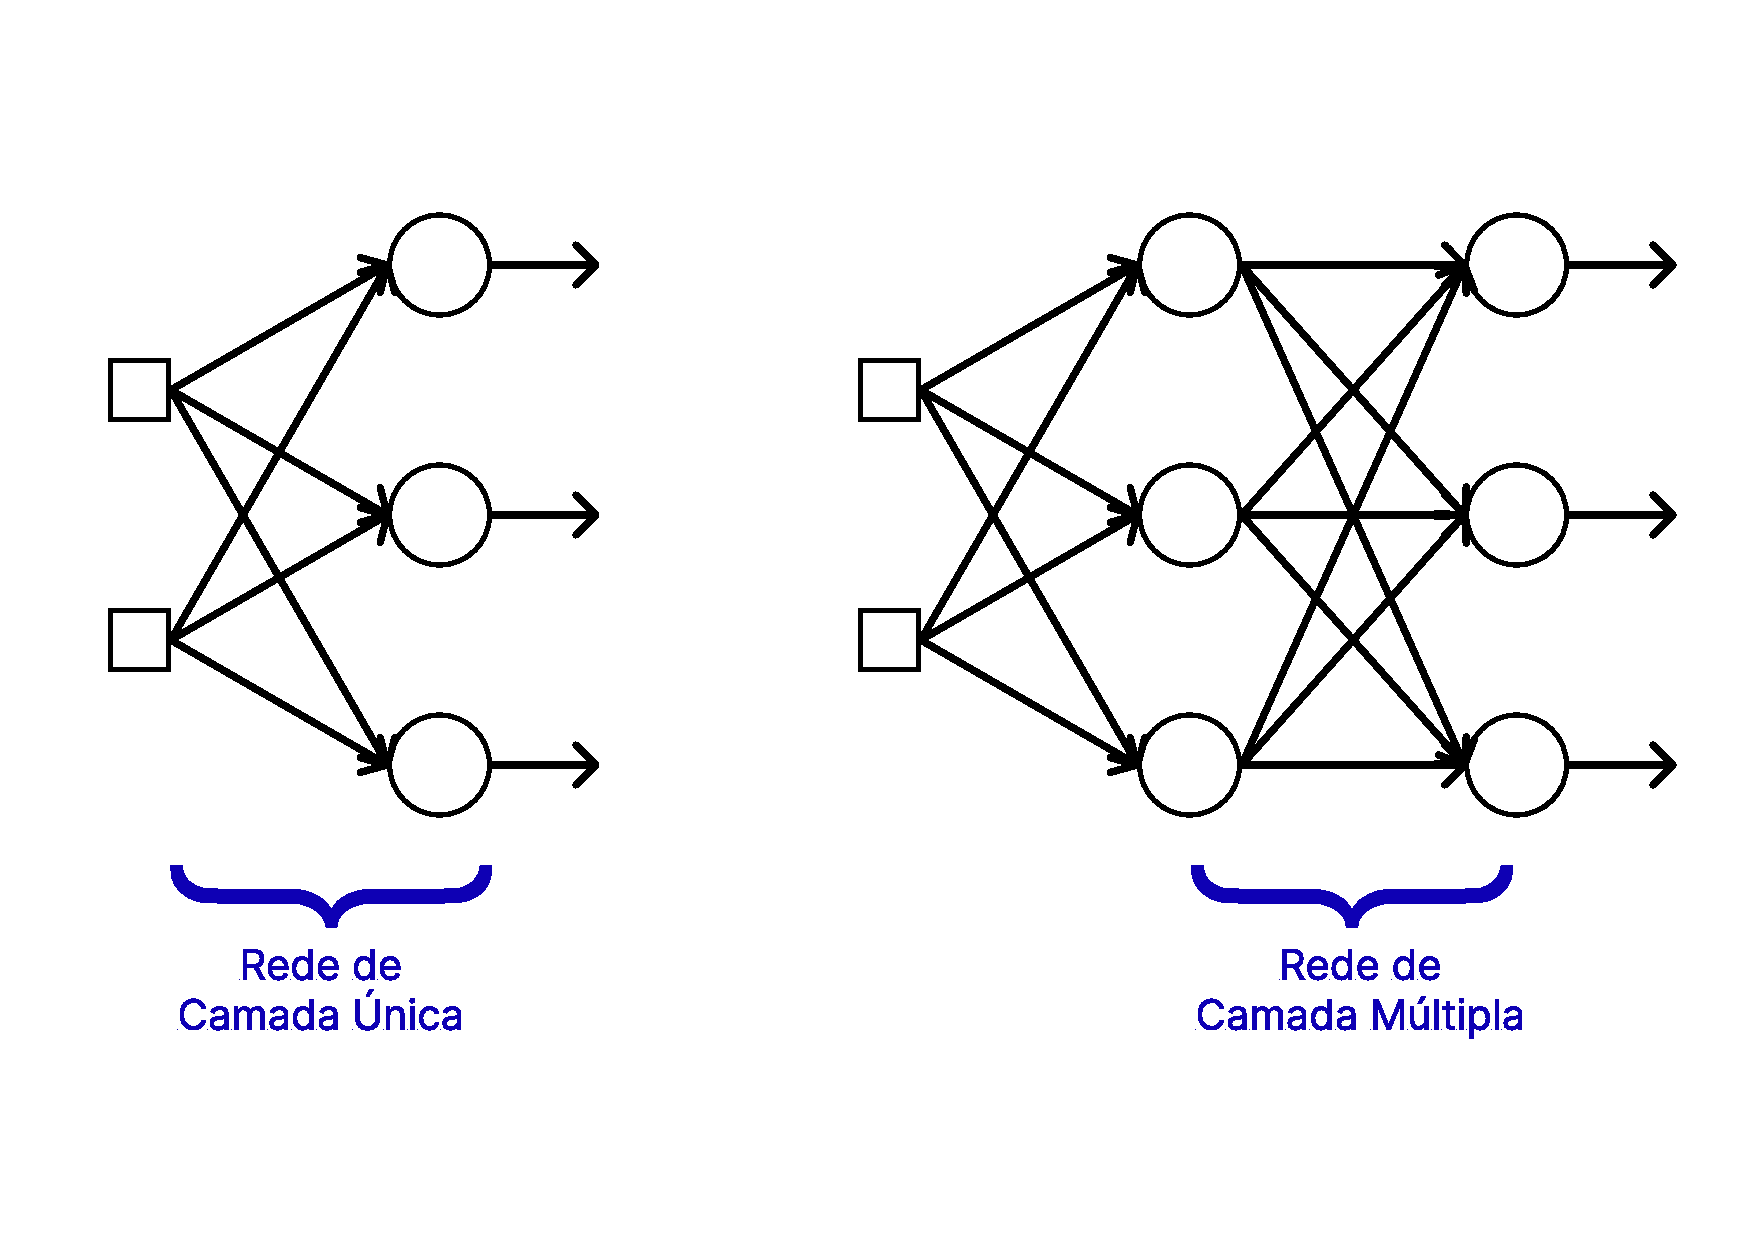
\includegraphics[scale=0.25]{figuras/network_layers.pdf}
		    \caption{Rede Camada Única e Múltipla \citep[adaptado de][]{haykin2009}}
	    \end{figure}
    \end{frame}

    \begin{frame}{Função de Ativação}
    % https://tex.stackexchange.com/questions/391369/two-column-items-with-titles-in-a-beamer
        \begin{columns}[onlytextwidth,t]
            \begin{column}{0.48\textwidth}
                \centering
                \textbf{Sigmóide (\textit{logit})}
                
                \begin{figure}
                    \includegraphics[scale=0.12]{figuras/sigmoid.pdf}
	            \end{figure}
	               
	            $f: \R \rightarrow (0,1)$ dada por 
	            \[f(x) := \frac{1}{1 + e^{-x}}\]
	            
            \end{column}

            \begin{column}{0.48\textwidth}
                \centering
                \textbf{Tangente Hiperbólica (\textit{tanh})}
            
                \begin{figure}
                     \includegraphics[scale=0.12]{figuras/tanh.pdf}
	            \end{figure}
	            
	            $f:\R \rightarrow (-1,1)$ dada por 
                \[f(x) := \frac{e^{x}-e^{-x}}{e^{x}+e^{-x}}\]
 
            \end{column}
        \end{columns}
    \end{frame}

    \begin{frame}{RNN - Redes Neurais Recorrentes}
        \begin{itemize}
            \item RNNs são um tipo de redes neurais criadas para processar séries temporais e outros tipos de dados sequenciais \citep{fan2021}.
        \end{itemize}
        \begin{figure}
           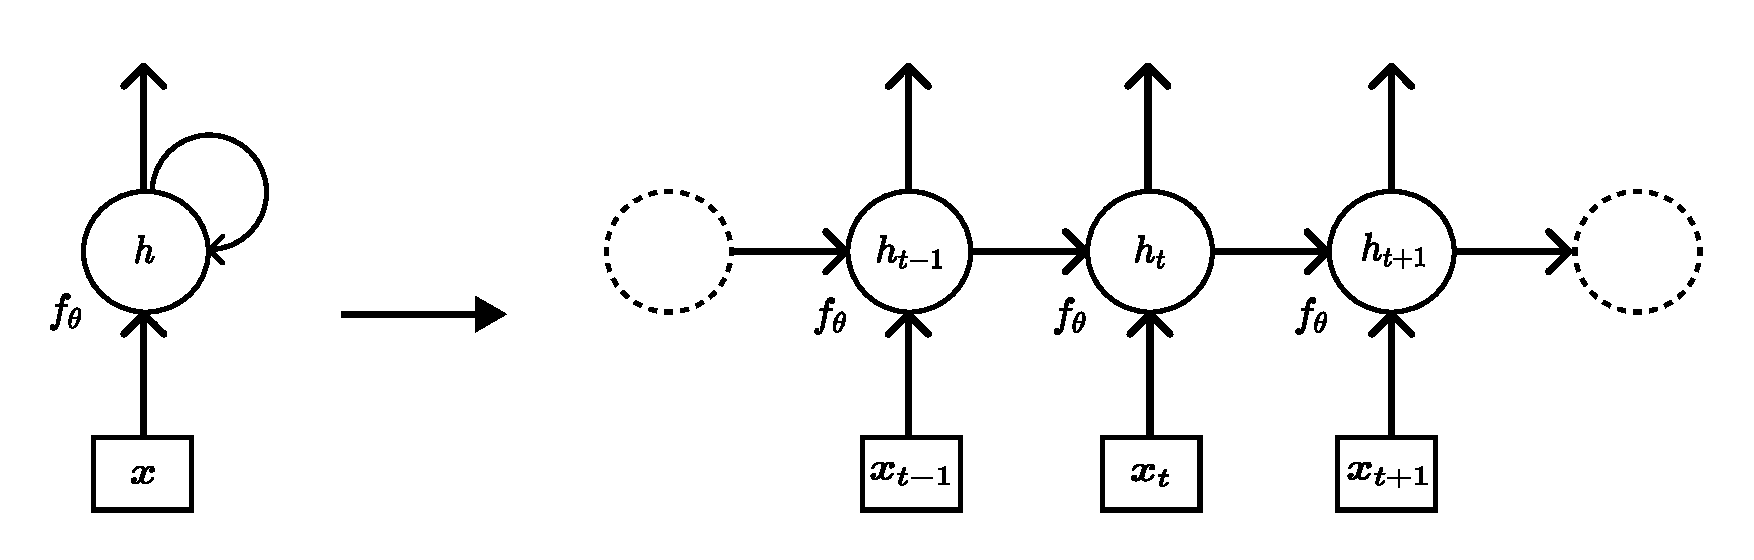
\includegraphics[scale=0.3]{figuras/rnn_hidden_state.pdf}
		    \caption{Diagrama de uma RNN \textit{Vanilla} \citep[adaptado de][]{goodfellow2016, kamath2019}}
	    \end{figure}
    \end{frame}

    \begin{frame}{LSTM - \textit{Long Short-Term Memory}}
        \begin{itemize}
            \justifying
            \item De acordo com \citet{goodfellow2016}, as LSTM fazem parte de uma classe de modelos chamada de RNN fechadas (\textit{gated RNN}).
            \item Os portões (\textit{gates}), que também são camadas da rede neural, controlam o fluxo de informação, mantendo ou descartando o estado oculto $\bs{h}_{t}$ a cada passo temporal \citep{kamath2019}.
            \item É uma das variantes de RNN desenvolvidas para contornar o problema de dissipação (ou explosão) do gradiente, que ocorre no ajuste da rede.
        \end{itemize}  
    \end{frame}
    
    \begin{frame}{LSTM - \textit{Long Short-Term Memory}}
       \begin{figure}
            \centering
            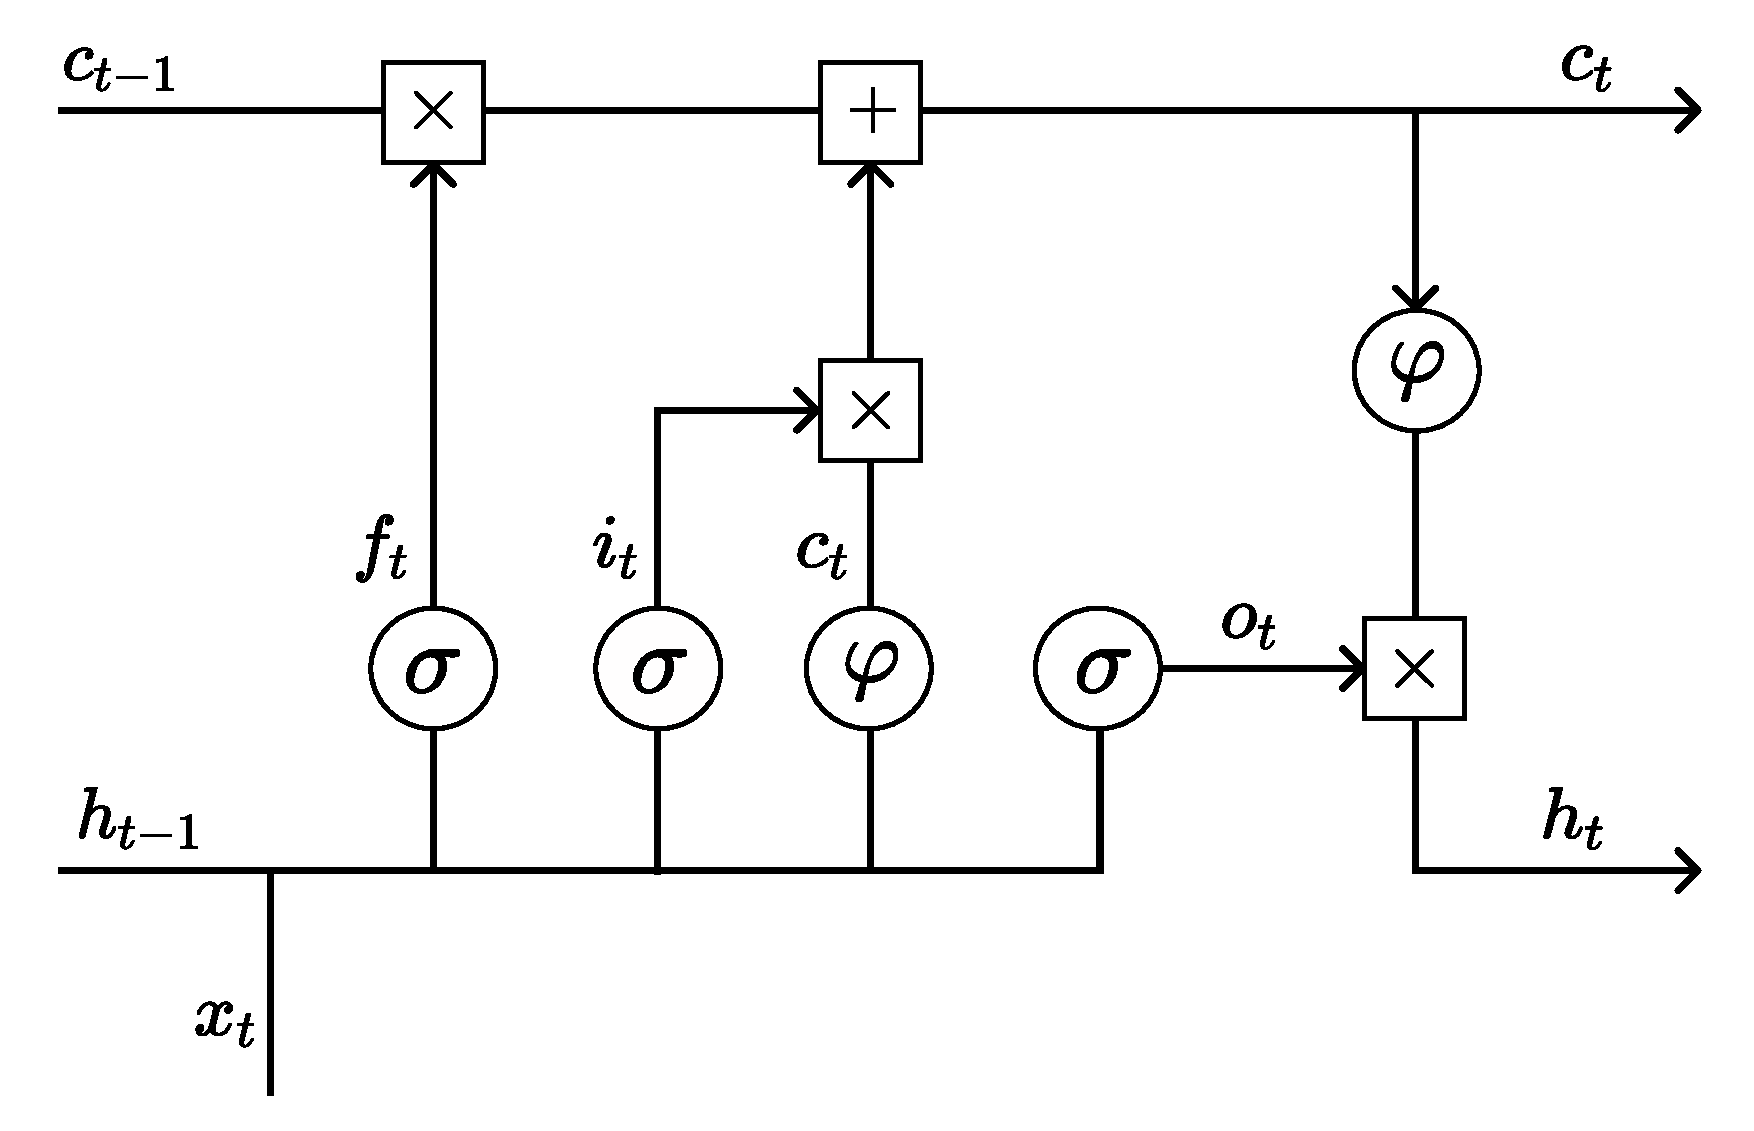
\includegraphics[scale=0.25]{figuras/lstm_cell.pdf}
	        \caption{Diagrama de uma LSTM. Considere $\sigma$ como a função de ativação \textit{logit} \citep[adaptado de][]{kamath2019}.}
        \end{figure}
    \end{frame}

    \begin{frame}{Ajustando uma RNA}
        \begin{itemize}
            \item função perda
            \item gradiente descendente e SGD
            \item taxa de aprendizagem
            \item retropropagação
        \end{itemize}
    \end{frame}

    \begin{frame}{PLN - Processamento de Linguagem Natural}
        \begin{itemize}
            \justifying
            \item aplicação de métodos estatísticos e computacionais para modelar e extrair informações da linguagem humana \citep{kamath2019};
            \item é importante testar os algoritmos em mais de uma linguagem, especialmente em linguagens com diferentes propriedades \citep{jurafsky2021}.
        \end{itemize}
    \end{frame}

    \begin{frame}{PLN - Entropia e Perplexidade}
        \begin{itemize}
            \item entropia
            \item entropia cruzada
            \item perplexidade
        \end{itemize}
    \end{frame}

    \begin{frame}{PLN - múltiplos}
        \begin{itemize}
            \item word embedding
            \item expressões regulares
            \item corpus
        \end{itemize}
    \end{frame}

    \begin{frame}{PLN - \textit{Word Embedding}}
        \begin{itemize}
            \item palavras (ou \textit{tokens}) são variáveis categóricas que precisam de uma codificação para que sejam utilizadas em um modelo estatístico
            \item duas possibilidades:
            \begin{itemize}
                \item \textit{one-hot encoding}:
                \item \textit{dense encoding}:
            \end{itemize}
            \item O principal benefício da \textit{dense encoding} é a capacidade de generalização, pois os valores do vetor denso são ajustáveis, possibilitando a captura de relações entre as diferentes palavras
        \end{itemize}
    \end{frame}

%Em PLN, as palavras (ou \textit{tokens}) são variáveis categóricas que precisam de uma codificação para que sejam utilizadas em um modelo estatístico. Seguem duas possibilidades:
%\begin{itemize}
%    \item \textit{one-hot encoding}: é criado uma variável indicadora (\textit{dummy}) para cada categoria.
%    \item \textit{dense encoding (feature embeddings)}: cada categoria é embutida em um vetor $d$-dimensional.
%\end{itemize}
%O principal benefício da \textit{dense encoding} é a capacidade de generalização, pois os valores do vetor denso são ajustáveis, possibilitando a captura de relações entre as diferentes palavras.


    \begin{frame}{Notação ABC}
        \vspace{0.1cm}
        \begin{itemize}
            \justifying
            \item Notação ABC é um sistema popular de notação musical baseada em texto para transcrever, publicar e compartilhar músicas, particularmente de forma \textit{online}. 
        \end{itemize}

        \begin{figure}
            \vspace{-0.5cm}
            \centering
            \includegraphics[scale=0.25]{figuras/abc_notation_example.pdf}
	        \caption{Exemplo de notação ABC convertendo em música.}
        \end{figure}
    \end{frame}

    \begin{frame}{\textit{Web Scraping}}
        \begin{itemize}
            \justifying
            \vspace{0.1cm}
            \item De acordo com \citet{lawson2015,patil2016}, envolve dois programas:
            \vspace{0.1cm}
            \begin{itemize}
                \item \textit{crawler}: sistematicamente coleta os dados da Internet;
                \item \textit{scraper}: extrai a informação relevante e armazena em uma base de dados.
            \end{itemize}
        \end{itemize}
        
        \begin{figure}
            \centering
            \includegraphics[scale=0.16]{figuras/spider_crawler.png}
	        \caption{\textit{Crawler} coletando páginas \textit{web}.}
        \end{figure}
        % https://www.scraping-bot.io/how-to-build-a-web-crawler/
    \end{frame}



\section{Modelagem}
    \begin{frame}{Bases de Dados}
        \begin{itemize}
            \item Irish
            \item ABC Notation
            \item tratamentos
        \end{itemize}
    \end{frame}

    \begin{frame}{Modelo}
        \begin{itemize}
            \item modelo
            \item arquitetura
            \item parâmetros e hiperparâmetros
        \end{itemize}
    \end{frame}
    
    \begin{frame}{Processo Gerador de Música}
        \begin{enumerate}
            \justifying
            \item construir um modelo com os devidos parâmetros; 
            \item fixado o modelo, carregam-se os pesos de um modelo similar ajustado previamente;
            \item fornecer uma sequência de caracteres inicial, no caso ``X:'';
            \item de forma iterativa, o modelo estima um novo elemento para compor a sequência até atingir um comprimento definido;
            \item extrair da sequência blocos de texto candidatos a músicas e, ao serem convertidos com sucesso, resultam em músicas.
        \end{enumerate}
    \end{frame}



\section{Resultados}
    \begin{frame}{Primeira Etapa - 32 modelos por base}
        bla bla bla
    \end{frame}

    \begin{frame}{Segunda Etapa - troca função de ativação}
        bla bla bla
    \end{frame}
    
    \begin{frame}{Geração de Músicas}
        \vspace{-1cm}
        \begin{columns}[onlytextwidth,t]
            \begin{column}{0.48\textwidth}
                \centering
                \textbf{Irish}: 24 músicas
                \vspace{0.1cm}
                \begin{itemize}
                    \item $idx=11$: 10 músicas
                    \begin{itemize}
                        \item \textit{logit}: 4 músicas
                        \item \textit{tanh}: 6 músicas
                    \end{itemize}
                    \vspace{0.25cm}
                    \item $idx=25$: 14 músicas
                    \begin{itemize}
                        \item \textit{logit}: 6 músicas 
                        \item \textit{tanh}: 8 músicas
                    \end{itemize}
                \end{itemize}
            \end{column}

            \begin{column}{0.48\textwidth}
                \centering
                \textbf{ABC Notation}: 14 músicas
                \vspace{0.1cm}
                \begin{itemize}
                    \item $idx=20$: 8 músicas
                    \begin{itemize}
                        \item \textit{logit}: 4 músicas
                        \item \textit{tanh}: 4 músicas
                    \end{itemize}
                    \vspace{0.25cm}
                    \item $idx=28$: 6 músicas
                    \begin{itemize}
                        \item \textit{logit}: 1 músicas
                        \item \textit{tanh}: 5 músicas
                    \end{itemize}
                \end{itemize}
            \end{column}
        \end{columns}
    \end{frame}
    
    \begin{frame}{Percepções sobre as Músicas}
        \begin{columns}[onlytextwidth,t]
            \begin{column}{0.48\textwidth}
                \centering
                \textbf{Irish}
                \vspace{0.1cm}
                \begin{itemize}
                    \item trechos similares
                    \item voz única
                    \item musicalmente plausível
                \end{itemize}
            \end{column}

            \begin{column}{0.48\textwidth}
                \centering
                \textbf{ABC Notation}
                \vspace{0.1cm}
                \begin{itemize}
                    \item mais variabilidade
                    \item voz múltipla
                    \item musicalmente plausível
                \end{itemize}
            \end{column}
        \end{columns}
        
        \vspace{1cm}
        Os comentários feitos referente às composições geradas são as percepções do autor com seu limitado conhecimento musical.
    \end{frame}



\section{Considerações Finais}
    \begin{frame}{Resumo}
        \begin{itemize}
            \justifying
            \item explorou-se o problema de composição automática de músicas; 
            \item investigou-se a sensibilidade dos modelos via modificação dos parâmetros;
            \item mediu-se impactos das mudanças via perplexidade;
            \item gerou-se novos arquivos \textit{.abc} que, quando possível, foram convertidos em músicas.
        \end{itemize}
    \end{frame}
    
    \begin{frame}{Extensões}
        \begin{itemize}
            \justifying
            \item modificar a arquitetura contemplando o aumento do número de camadas;
            \item explorar outros perfis de redes, como a \textit{transformer} \citep{vaswani2017};
            \item analisar detalhadamente características musicais das composições.
        \end{itemize}
    \end{frame}



%
    \begin{frame}[allowframebreaks]
        \frametitle{Referências}
        \bibliographystyle{apalike}
        \bibliography{biblio}
    \end{frame}


\end{document}